The Standard Model (SM), the theoretical framework which describes fundamental particles
and their interactions, provides understanding for a wealth of results from accelerator-based
and cosmic ray-based experiments, in many cases with great accuracy.
The recent discovery of a Higgs particle, a long sought particle that is responsible for
the electroweak symmetry 
breaking, emphasizes the success of the theory.

However, we are fast approaching a time where the Standard Model may break down,
where observations of inexplicable experimental results will call for additional theoretical 
interpretations. Significant pieces of the Standard Model still remain challenging: the hierarchy
problem, the unification of the fundamental forces at very small distances and their possible
connection to gravity, the dark matter and dark energy hypotheses etc.
The issues we have already encountered at the energy scales available experimentally 
hint at some grander underlying structure of nature, which is yet to be found.

% More intro needed

Used throughout is the system of units in which $\hbar=c=1$.


\section{The Standard Model}

The Standard Model is a quantum field theory of elementary particles that describes 
three of the four fundamental interactions: 
the electromagnetic, the weak, and the strong interactions. The fourth fundamental
interaction, the gravity, 
is not a part of the model as no quantum theory of gravity exists to this date. 
The theory is described in detail elsewhere, e.g. \cite{Tully:1417476}, 
but a brief overview is given here.

In SM each particle is described
in terms of a dynamical field that pervades the space-time, while the internal dynamics 
and kinematics are controlled by a relativistically invariant Lagrangian.
What defines the Standard Model are the three local gauge symmetries of the Lagrangian
corresponding to three fundamental interactions.
One should note however, that particle mass and electric charge, 
which are well known properties from 
classical physics, are highly non-obvious quantities in the Standard Model. They
will be re-introduced together with the mechanism of electroweak symmetry breaking, however
at this point,
all elementary particles are assumed massless and only the possible quantum numbers
and degrees of freedom of particle states are investigated.

The existence of an interaction is reflected in the quantum numbers of the elementary
particles, while an interaction itself can be viewed as a transformation between particle states
into one another in a manner similar to a rotation, but within an internal space of the interaction.
The Standard Model Lagrangian is assumed invariant under the following symmetry group:
\begin{equation}
SU(3)_C \times SU(2)_L \times U(1)_Y
\label{eqn:symSM}
\end{equation}
where $C$ denotes the colour interaction, $L$ the weak isospin interaction 
that acts only on the left-handed part of the spinors, and $Y$ is the hypercharge
interaction.

The smallest non-trivial representation of the weak isospin interaction is
a two-component doublet of particles with three generators
of rotations in the isospin space denoted as $W^i$ and i=1,2,3.
Therefore, there is an "up" and "down" type in each weak isospin doublet of elementary particles.
Both quarks and leptons are arranged into doublets of weak isospin, the up quarks ($u$, $c$, $t$)
are matched to down quarks ($d$, $s$, $b$), and the leptons ($e$, $\mu$, $\tau$) are matched
to neutrinos ($\nu_e$, $\nu_{\mu}$, $\nu_{\tau}$). The weak isospin doublets of quarks and leptons
are presented in Figure \ref{fig:parttable}.  
The hypercharge $Y$ has every similarity to electric charge, with the exception of the
charge assignments to the elementary particles so to preserve indistinguishability of the components
of weak isospin doublets.

The sub-symmetry $SU(2)_L \times U(1)_Y$ describes the electroweak sector of the SM with the 
following Lagrangian:
\begin{equation}
\mathcal{L}_\mathrm{EW} = \sum_\psi\bar\psi\gamma^\mu \left(i\partial_\mu-g^\prime{1\over2}YB_\mu-g{1\over2}\vec\tau_\mathrm{L}\vec W_\mu\right)\psi
\label{eqn:LagrEWK}
\end{equation}
where $B_{\mu}$ is the U(1) gauge field; $Y$ is the hypercharge, the generator of 
the U(1) group; $\vec{W}_\mu$ is the three-component SU(2) gauge field; $\vec{\tau}_\mathrm{L}$
 are the Pauli matrices, infinitesimal generators of the SU(2) group. 
The subscript $L$ indicates that they only act on left-handed fermions; $g^{'}$ and $g$
 are coupling constants.



The gauge symmetry associated with the colour (strong) interaction is a three-dimensional special
unitary transformation SU(3). The internal space of the strong interaction has a smallest
non-trivial representation given by a triplet of states, denoted as colors: red, blue, and green,
and a set of eight generators of rotation. Such a color triplet is called a quark, with the
three colour states being indistinguishable, while the
eight carriers of the strong interaction are called gluons. 



\begin{equation}
\mathcal{L}_{QCD} = i\overline U (\partial_\mu-ig_sG_\mu^a T^a)\gamma^\mu U + i\overline D (\partial_\mu-i g_s G_\mu^a T^a)\gamma^\mu D.
\label{eqn:LagrQCD}
\end{equation}

$G_\mu^a$ is the SU(3) gauge field containing the gluons, $\gamma^\mu$ are the Dirac matrices,
 D and U are the Dirac spinors associated with up- and down-type quarks, and $g_s$ 
is the strong coupling constant.

\begin{figure}
\centering
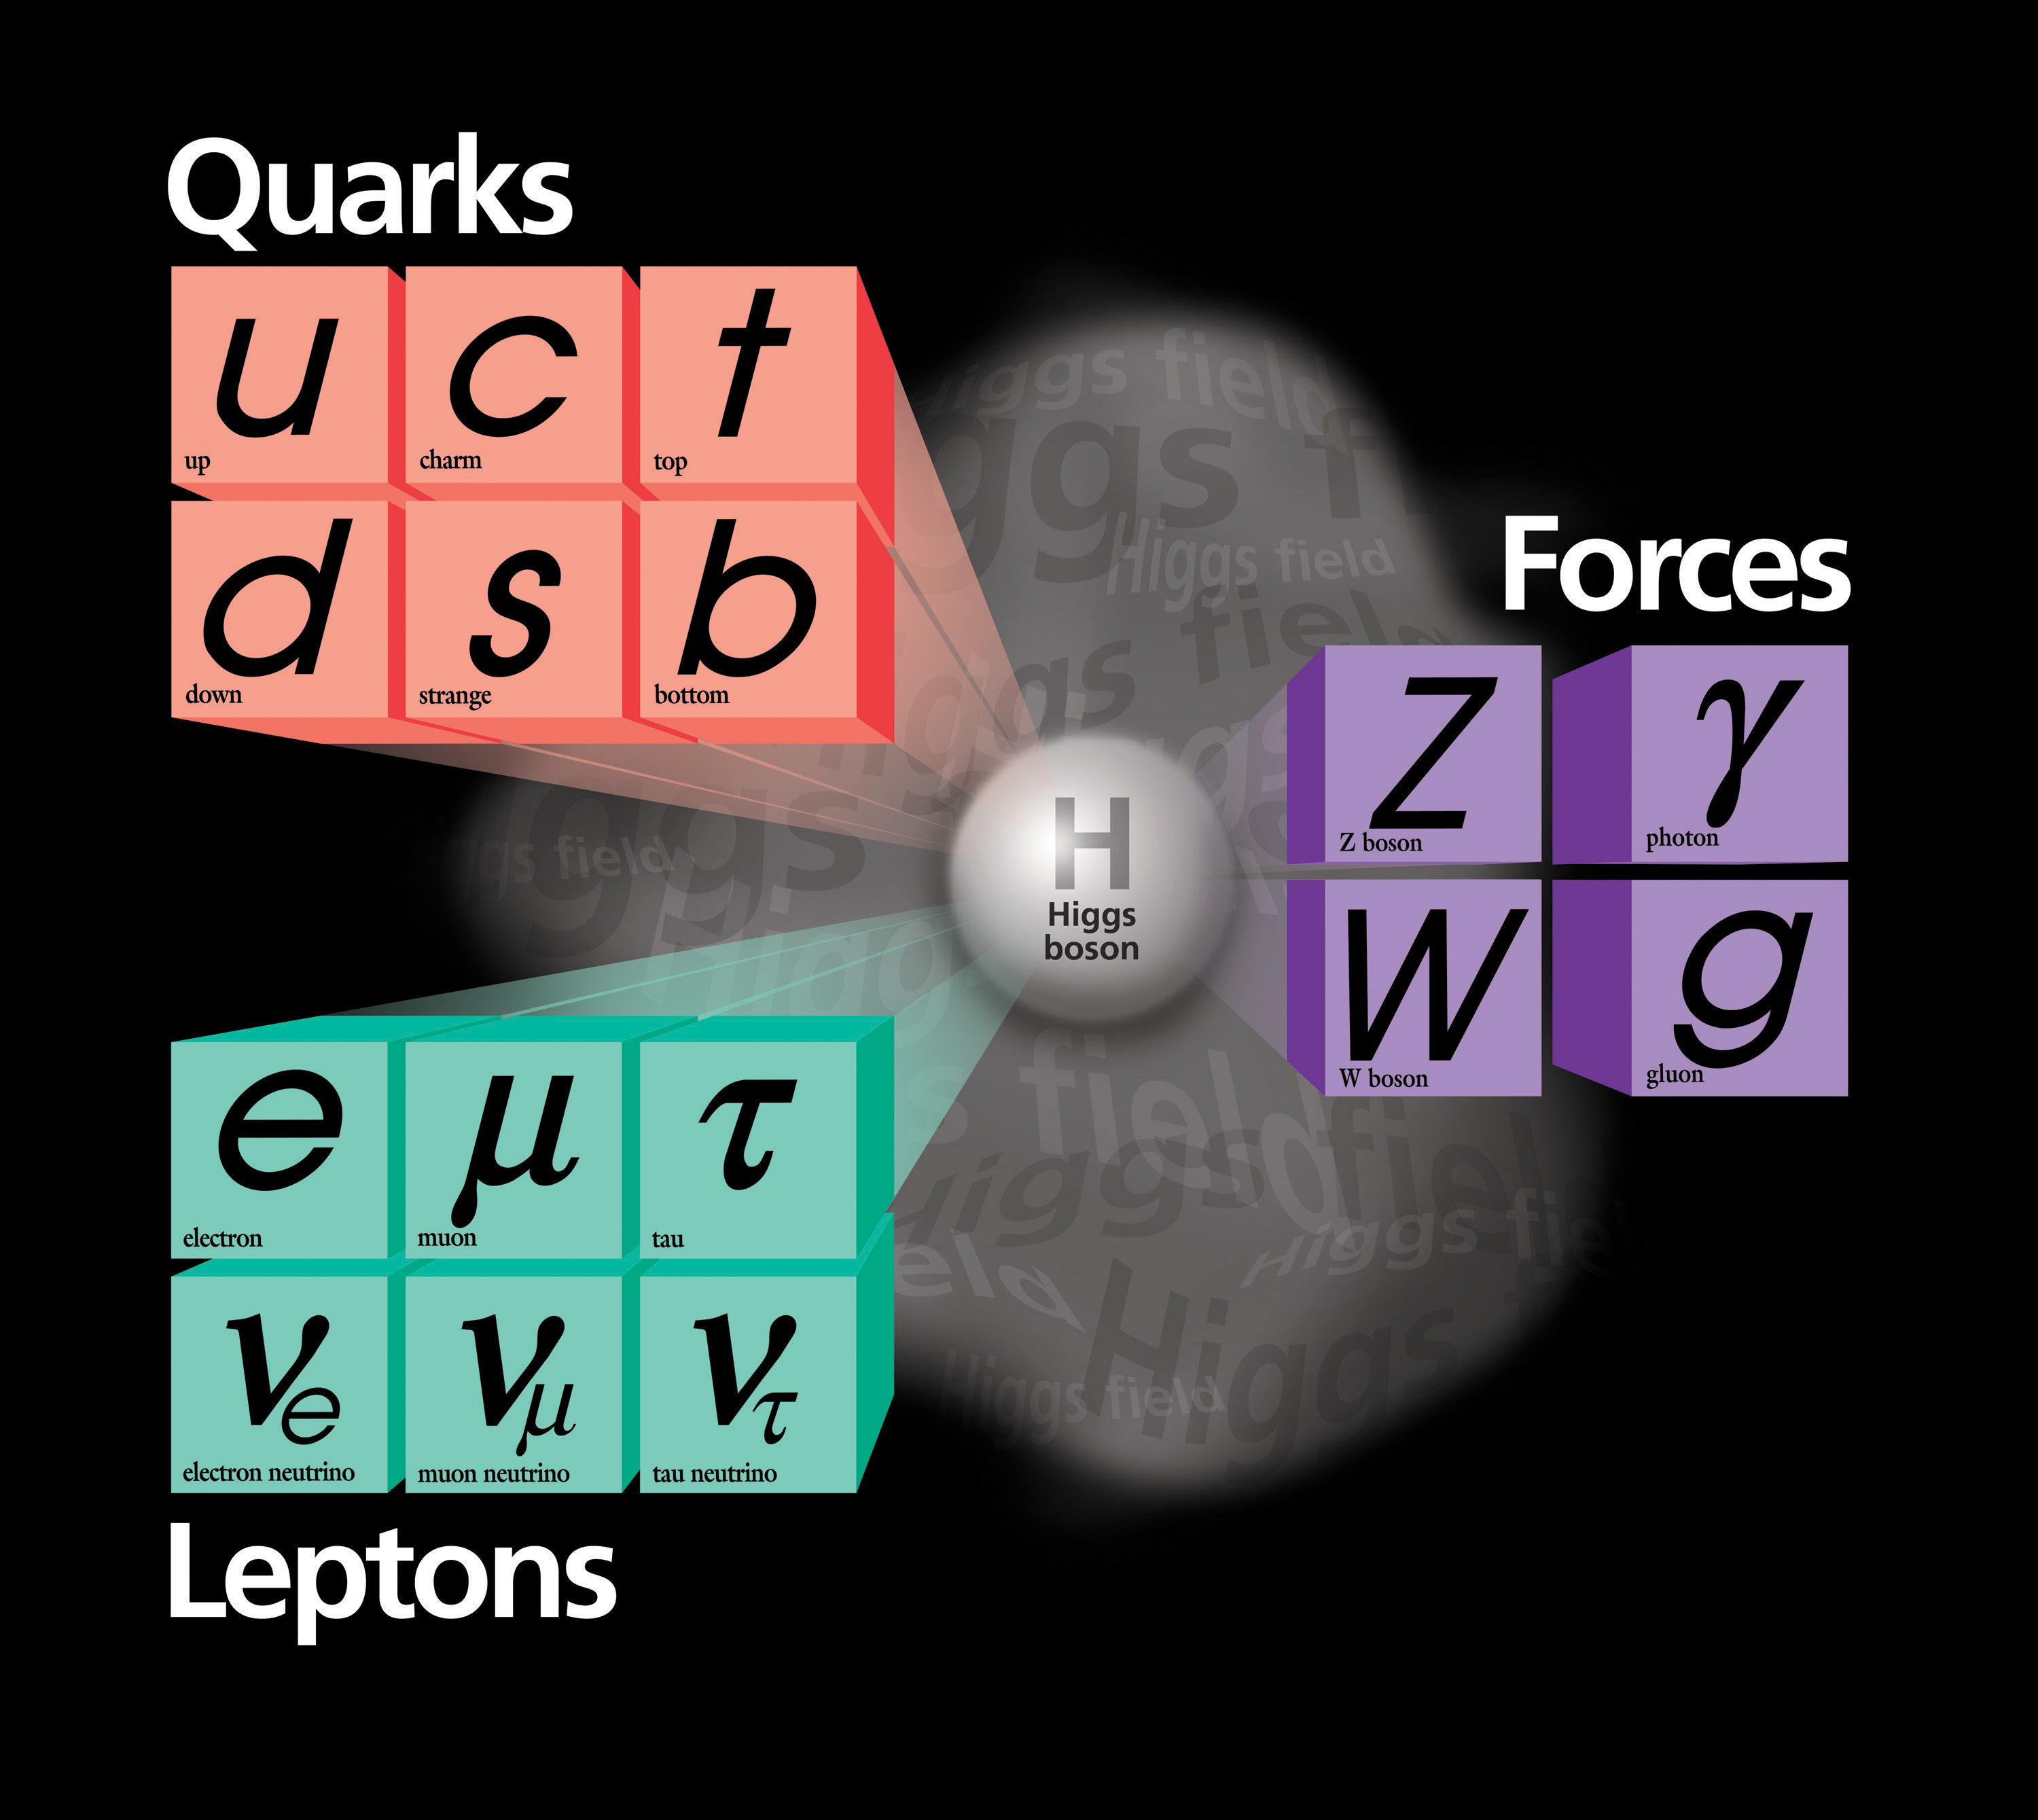
\includegraphics[width=0.6\textwidth]{plots/intro/Higgs_SM.jpeg}
\caption{Table of elementary particles: quarks and leptons (spin-1/2) on the left,
the gauge bosons (spin-1) on the right, in the center the Higgs boson (spin-0).
\label{fig:parttable}}

\end{figure}

We know that within each of the weak isospin doublets, both particles 
differ in terms of their
mass and electric charge, making them distinguishable,
 therefore the weak isospin interaction is
 not an observed symmetry of nature, but it was clearly present
in some form given the structure of the particles table. 
In order to explain the physically observed masses and charges of elementary
 particles we need to introduce the electroweak symmetry breaking, a central concept
of the Standard Model that transforms the
weak isospin and hypercharge interactions into the well known weak and electromagnetic forces.



\subsection{Higgs Mechanism}

What happens if a particle field takes on a non-zero expectation value in vacuum? Depending on the
quantum numbers of the non-zero field, the vacuum will not necessarily be invariant under
all symmetries of the Lagrangian. That's what is postulated by the Higgs mechanism, where
an existence of a scalar field, with non-zero vacuum expectation value
reduces the gauge symmetries of the physical 
vacuum from $SU(3)_C \times SU(2)_L \times U(1)_Y$
down to $SU(3)_C \times U(1)_{EM}$. Therefore leaving the physical vacuum invariant under
only the color and electric charges. 
The $U(1)_{EM}$ symmetry group requires the existence of a massless
gauge boson, the photon ($\gamma$), as the carrier of electromagnetic force.
After symmetry breaking the gauge bosons mix to form weak and electromagnetic fields.



\begin{figure}[htbp]
\centering
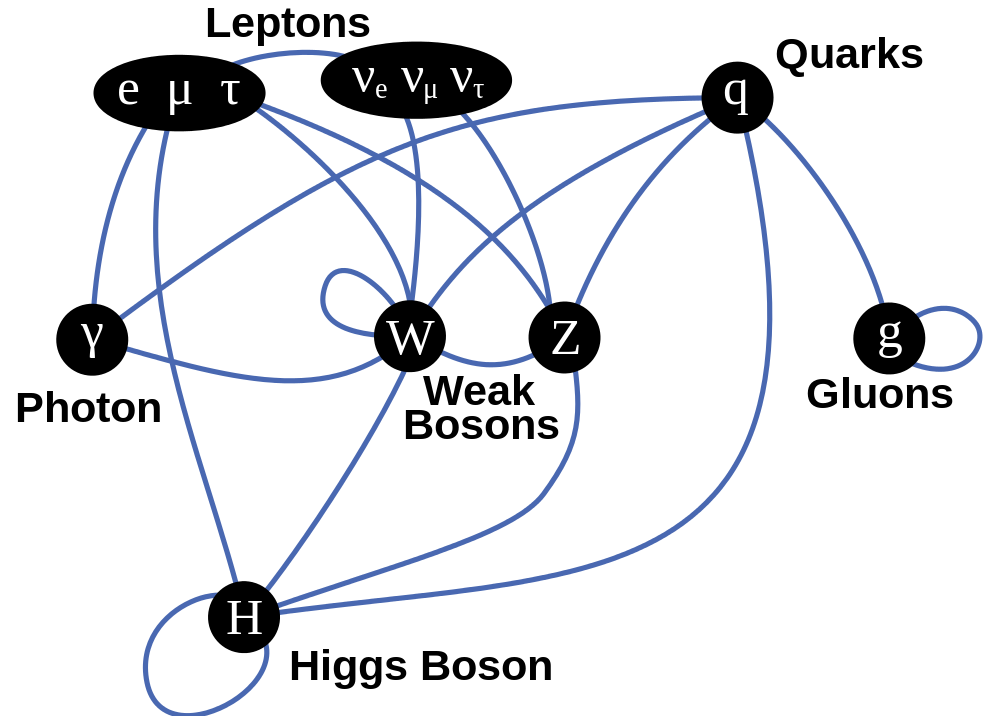
\includegraphics[width=0.7\textwidth]{plots/intro/eleparticles.png}
\caption{Fundamental particles of the Standard Model. The lines connecting the particles
indicate a presence of an interaction between them. \label{fig:eleparticles}}
\end{figure}

